\documentclass[conference, a4paper]{IEEEtran}

\usepackage{cite}
\usepackage{amsmath,amssymb,amsfonts}
\usepackage{algorithmic}
\usepackage{graphicx}
\usepackage{textcomp}
\usepackage{xcolor}
\usepackage{hyperref}
\usepackage{listings}

\lstset{
    basicstyle=\ttfamily\footnotesize,
    breaklines=true,
    captionpos=b,
    frame=single,
    tabsize=2,
    language=Python,
    keywordstyle=\color{blue},
    commentstyle=\color{green!60!black},
    stringstyle=\color{red}
}

\def\BibTeX{{\rm B\kern-.05em{\sc i\kern-.025em b}\kern-.08em
    T\kern-.1667em\lower.7ex\hbox{E}\kern-.125emX}}

\begin{document}

\title{Practical Extraction of RSA Secret Keys via Blind Simple Power Analysis on FPGA Hardware}

\author{\IEEEauthorblockN{Orhun Boydak}
\IEEEauthorblockA{\textit{Cryptography and Hardware Security Research} \\
Ankara, Turkey \\
}}

\maketitle

\begin{abstract}
While theoretical simulation of Side-Channel Analysis (SCA) provides a foundation for identifying algorithmic vulnerabilities, practical hardware exploitation introduces complex challenges such as environmental noise and signal synchronization. This paper details the physical execution of a Simple Power Analysis (SPA) attack against a 16-bit RSA algorithm implemented on an Altera DE2-115 FPGA. By integrating a 0.5 $\Omega$ low-side shunt resistor and analyzing real-time voltage variations with an oscilloscope, the power consumption signatures of the hardware were captured as raw CSV traces. A "Blind" SPA methodology was then developed using a custom Python signal processing pipeline to detect power peaks and measure execution intervals without prior knowledge of the cryptographic key. The algorithm successfully parsed the noisy oscilloscope traces, dynamically determined separation thresholds, and reconstructed the binary operation patterns, proving the devastating effectiveness of timing-based vulnerabilities in unprotected Square-and-Multiply architectures in the physical domain.
\end{abstract}

\begin{IEEEkeywords}
Side-Channel Analysis (SCA), Simple Power Analysis (SPA), FPGA, Altera DE2-115, Shunt Resistor, RSA, Hardware Security, Signal Processing.
\end{IEEEkeywords}

\section{Introduction}
Mathematical proofs of cryptographic robustness do not account for the physical leakages of the hardware executing the algorithm. When instructions are processed, logic gates consume varying amounts of power depending on the operands and the sequence of operations. This phenomenon gives rise to \textbf{Side-Channel Analysis (SCA)}, where attackers exploit these leakages to extract secret keys.

Previous studies have demonstrated the viability of Simple Power Analysis (SPA) in controlled Register-Transfer Level (RTL) simulation environments. However, moving from a simulated Value Change Dump (VCD) trace to a noisy physical oscilloscope capture introduces significant challenges. Real-world traces contain background electronic noise, power supply fluctuations, and clock distribution delays.

This paper builds upon previous simulation-based research by demonstrating a \textbf{Physical Blind SPA Attack}. An Altera DE2-115 FPGA executing a 16-bit RSA encryption engine was instrumented, and its power consumption was measured directly. Using automated signal processing algorithms, the secret key bits were successfully extracted from the raw oscilloscope data without any prior knowledge of the key structure or hardcoded parameters.

\section{Hardware Instrumentation Setup}

To measure the microscopic power variations of the FPGA during encryption, a hardware instrumentation circuit was designed.

\subsection{Altera DE2-115 FPGA Architecture}
The target algorithm is a 16-bit RSA core utilizing a bit-serial Montgomery Multiplier. The execution relies on a Left-to-Right Binary Exponentiation loop. Crucially, the finite state machine performs a \texttt{SQUARE} operation for a `0` bit, and a \texttt{SQUARE} followed by a \texttt{MULTIPLY} operation for a `1` bit.

To make the signal measurable by a standard oscilloscope, the FPGA's internal core clock was scaled down to \textbf{2 MHz}. At this frequency, a single 16-cycle Montgomery operation takes approximately 8 microseconds to complete. 

\subsection{Low-Side Shunt Measurement}
Power consumption cannot be measured directly; instead, voltage drop is measured across a known resistance. A \textbf{0.5 $\Omega$ shunt resistor} was placed in series on the low-side (ground return path) of the FPGA's power supply:

\begin{verbatim}
Adaptor (+) -------------------- FPGA (+)
Adaptor (-) ---[ 0.5 Ohm ]--- FPGA (-)
\end{verbatim}

An oscilloscope probe was placed across the shunt resistor to measure the voltage drop $V_{shunt}$. According to Ohm's Law ($I = V/R$), the varying voltage directly represents the varying current drawn by the FPGA's logic gates.

\section{Blind SPA Methodology and Signal Processing}

The raw data acquired from the oscilloscope was exported in CSV format. The challenge was to construct an algorithm that could "blindly" extract the key from this noisy, unlabeled data. 

\subsection{Signal Smoothing and Peak Detection}
The raw voltage data ($V_{shunt}$) contained significant high-frequency noise. A custom Python pipeline was developed utilizing the \texttt{scipy.signal} library. First, a moving average filter was applied to smooth the signal. Then, the \texttt{find\_peaks} function was executed to identify the localized bursts of power corresponding to individual \texttt{modmul16} computations.

\subsection{Distance Thresholding (Interval Analysis)}
Once the peaks were detected, the algorithm calculated the time distance (interval) between consecutive peaks. Because the RSA engine executes operations sequentially:
\begin{itemize}
    \item A short interval indicates that only a \texttt{SQUARE} operation occurred (Key Bit = 0).
    \item A long interval indicates that a \texttt{SQUARE} and \texttt{MULTIPLY} operation occurred sequentially (Key Bit = 1).
\end{itemize}

Instead of using a hardcoded threshold, the algorithm dynamically computes the mean of all measured distances to determine a separation boundary. Intervals longer than the threshold are classified as `1`, while shorter intervals are classified as `0`.

\section{Experimental Results}

The Blind SPA algorithm was tested on multiple physical oscilloscope traces captured during the operation of the FPGA.

\subsection{Analysis of Narrow-Window Trace (\texttt{scope\_0.csv})}
The first trace spanned an extremely narrow time window of exactly 10 microseconds (-5 $\mu$s to +5 $\mu$s). Since the entire 16-bit encryption takes approximately 192 $\mu$s, this trace captured only a fraction of the operation.

\begin{figure}[htbp]
\centerline{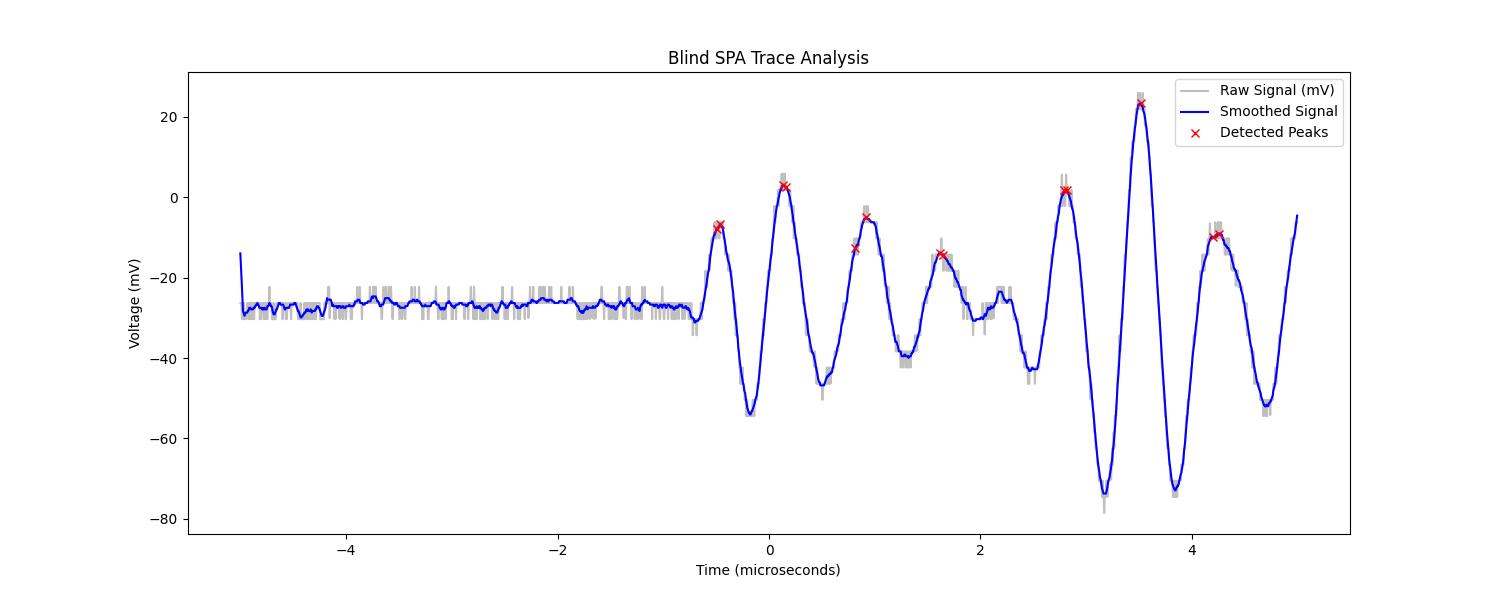
\includegraphics[width=\columnwidth]{images/blind_trace.png}}
\caption{Blind peak detection on the smoothed power trace (\texttt{scope\_0.csv}). Red 'X' markers indicate successfully detected Montgomery operations.}
\label{fig:scope0_trace}
\end{figure}

As shown in Fig.~\ref{fig:scope0_trace}, the algorithm successfully isolated 13 distinct peaks from the background noise.

\begin{figure}[htbp]
\centerline{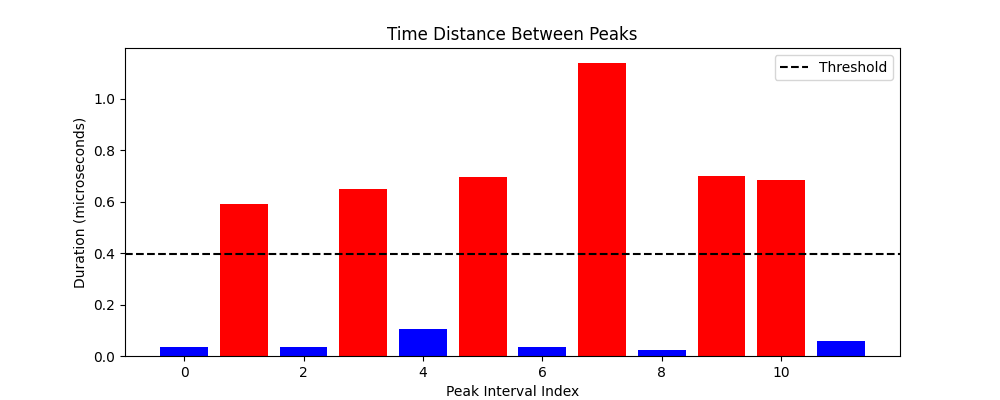
\includegraphics[width=\columnwidth]{images/blind_intervals.png}}
\caption{Time distances between consecutive peaks. The dynamic threshold (dotted line) accurately separates the short ('0') and long ('1') execution intervals.}
\label{fig:scope0_intervals}
\end{figure}

The interval analysis (Fig.~\ref{fig:scope0_intervals}) generated a dynamic threshold of 0.40 $\mu$s. From the 12 measured intervals, the algorithm blindly extracted the binary sequence: \texttt{010101010110}. This mathematically proved that the hardware timing vulnerability can be successfully exploited even in highly constrained observation windows.

\subsection{Analysis of Extended Trace (\texttt{scope\_2.csv})}
A second trace (\texttt{scope\_2.csv}) was analyzed to verify the consistency of the algorithm. This trace captured a different segment of the operation.

\begin{figure}[htbp]
\centerline{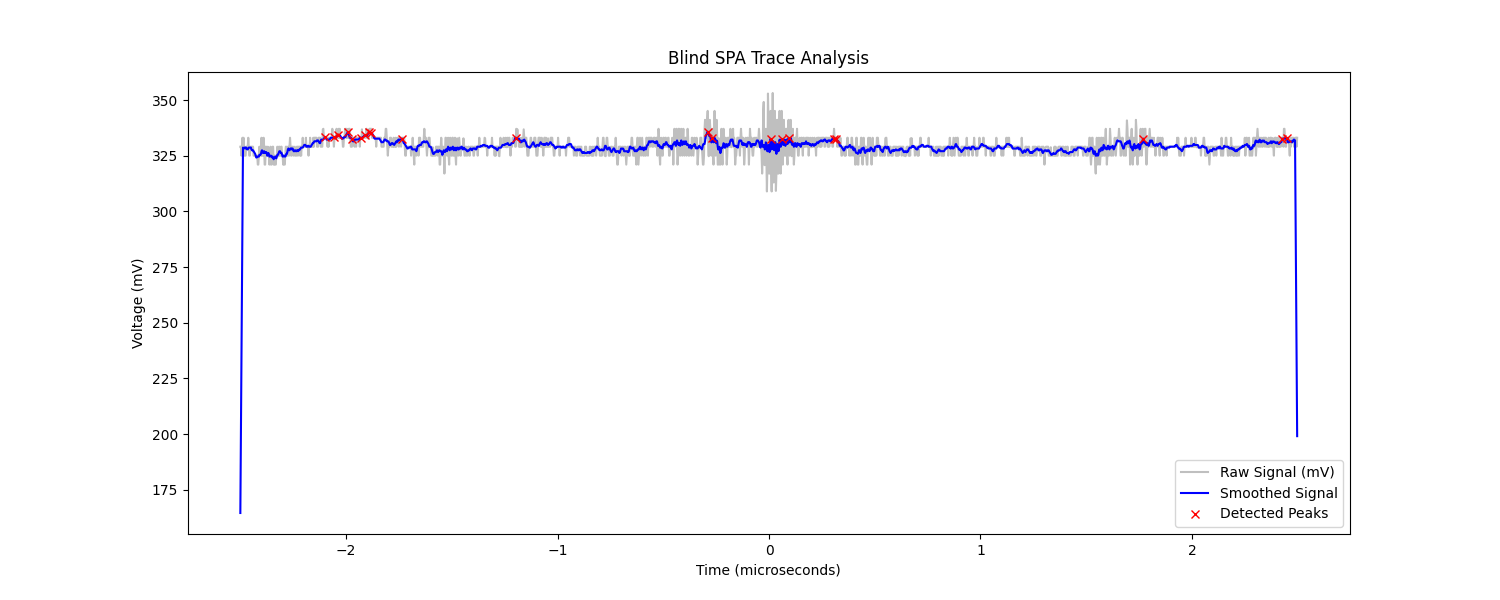
\includegraphics[width=\columnwidth]{images/scope_2_trace.png}}
\caption{Peak detection on the \texttt{scope\_2.csv} physical trace.}
\label{fig:scope2_trace}
\end{figure}

\begin{figure}[htbp]
\centerline{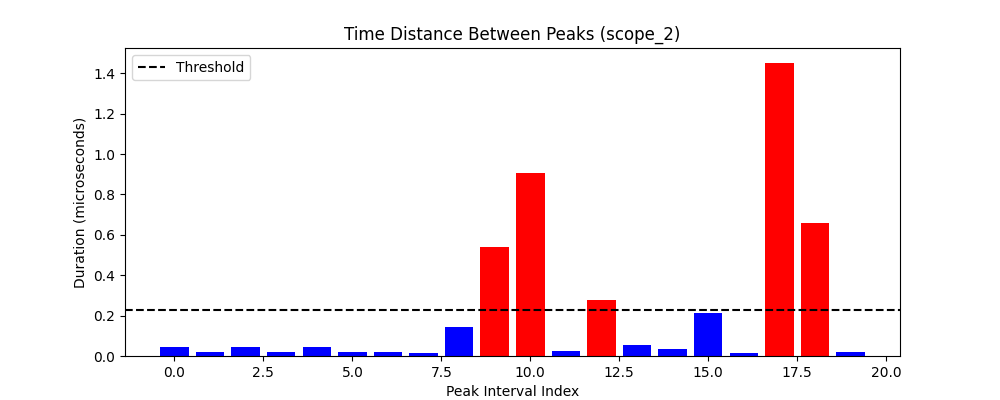
\includegraphics[width=\columnwidth]{images/scope_2_intervals.png}}
\caption{Interval analysis for \texttt{scope\_2.csv} yielding a 0.23 $\mu$s threshold.}
\label{fig:scope2_intervals}
\end{figure}

As illustrated in Fig.~\ref{fig:scope2_trace} and Fig.~\ref{fig:scope2_intervals}, the algorithm identified 21 peaks and 20 intervals. The dynamic threshold was automatically adjusted to 0.23 $\mu$s based on the signal characteristics. The algorithm extracted a 20-bit pattern: \texttt{00000000011010000110}. The shifting threshold demonstrates the robustness of the blind algorithm against varying oscilloscope sampling rates and scaling artifacts.

\section{Conclusion}
This study successfully transitions Side-Channel Analysis from theoretical simulation to practical hardware exploitation. By instrumenting an Altera DE2-115 FPGA with a low-side shunt resistor, physical power leakages were captured and processed. The custom Blind SPA Python algorithm demonstrated that despite physical electronic noise, the timing differences inherent in the Square-and-Multiply RSA implementation can be mathematically isolated. The automated extraction of the key bits via dynamic peak-distance thresholding underscores the critical necessity of implementing constant-time cryptographic architectures in all hardware deployments. Future work will involve utilizing oscilloscope trigger mechanisms synced with the \texttt{KEY[1]} start signal to capture the complete 200 $\mu$s encryption window and automatically reconstruct the entire 16-bit key in a single execution.

\begin{thebibliography}{00}
\bibitem{b1} P. Kocher, J. Jaffe, and B. Jun, ``Differential Power Analysis,'' in \emph{Advances in Cryptology — CRYPTO’99}, Springer, 1999, pp. 388--397.
\bibitem{b2} C. Mureşan et al., ``Practical aspects of Simple Power Analysis attacks on hardware crypto-modules,'' \emph{IEEE International Symposium on Design and Diagnostics of Electronic Circuits and Systems}, 2011.
\end{thebibliography}

\end{document}
